\documentclass[12pt]{amsart}
%prepared in AMSLaTeX, under LaTeX2e
\addtolength{\oddsidemargin}{-1.1in} 
\addtolength{\evensidemargin}{-1.1in}
\addtolength{\topmargin}{-.9in}
\addtolength{\textwidth}{1.75in}
\addtolength{\textheight}{1.75in}

\renewcommand{\baselinestretch}{1.05}

\usepackage{verbatim} % for "comment" environment

\usepackage{palatino}

\usepackage[final]{graphicx}

\usepackage{tikz}
\usetikzlibrary{positioning}

\usepackage{bm,enumitem,xspace,fancyvrb}

\newtheorem*{thm}{Theorem}
\newtheorem*{defn}{Definition}
\newtheorem*{example}{Example}
\newtheorem*{problem}{Problem}
\newtheorem*{remark}{Remark}

\DefineVerbatimEnvironment{mVerb}{Verbatim}{numbersep=2mm,frame=lines,framerule=0.1mm,framesep=2mm,xleftmargin=4mm,fontsize=\footnotesize}

% macros
\usepackage{amssymb}
\newcommand{\bA}{\mathbf{A}}
\newcommand{\bB}{\mathbf{B}}
\newcommand{\bE}{\mathbf{E}}
\newcommand{\bF}{\mathbf{F}}
\newcommand{\bJ}{\mathbf{J}}

\newcommand{\bb}{\mathbf{b}}
\newcommand{\bc}{\mathbf{c}}
\newcommand{\bd}{\mathbf{d}}
\newcommand{\bi}{\mathbf{i}}
\newcommand{\bj}{\mathbf{j}}
\newcommand{\bk}{\mathbf{k}}
\newcommand{\br}{\mathbf{r}}
\newcommand{\bv}{\mathbf{v}}
\newcommand{\bw}{\mathbf{w}}
\newcommand{\bx}{\mathbf{x}}

\newcommand{\bzero}{\bm{0}}

\newcommand{\eps}{\epsilon}
\newcommand{\grad}{\nabla}
\newcommand{\ip}[2]{\ensuremath{\left<#1,#2\right>}}
\newcommand{\lam}{\lambda}
\newcommand{\lap}{\triangle}

\newcommand{\Null}{\operatorname{null}}
\newcommand{\rank}{\operatorname{rank}}
\newcommand{\range}{\operatorname{range}}
\newcommand{\trace}{\operatorname{tr}}

\newcommand{\RR}{\mathbf{R}}

\newcommand{\ZZ}{\mathbb{Z}}

\newcommand{\prob}[1]{\bigskip\noindent\textbf{#1.}\quad }
\newcommand{\exer}[2]{\prob{Exercise #2 on page #1}}

\newcommand{\pts}[1]{(\emph{#1 pts}) }
\newcommand{\epart}[1]{\bigskip\noindent\textbf{(#1)}\quad }
\newcommand{\ppart}[1]{\,\textbf{(#1)}\quad }

\newcommand{\Matlab}{\textsc{Matlab}\xspace}
\newcommand{\ds}{\displaystyle}


\begin{document}
\scriptsize \noindent Math 314 Linear Algebra (Bueler) \hfill 21 March 2022 \fbox{\emph{Not to be turned in!}}
\normalsize\medskip

\Large\centerline{\textbf{Worksheet: 4 curve-fitting problems}}
\medskip
\normalsize

\thispagestyle{empty}
\begin{quote}
\quad The four graphs below show solutions of data-fitting problems.  The curve goes exactly through the data in problem \textbf{1}.  It comes as close to the data as possible, in the least-squares sense, in problems \textbf{2}, \textbf{3}, \textbf{4}.  We think of this as solving a linear system, but in fact when the number of points exceeds the number of parameters the system is over-determined.  The system is ``solved'' via the normal equations as in \S4.3:
  $$\text{``}A\bv=\bb\text{''} \qquad \stackrel{\text{replaced by}}{\to} \qquad A^\top A \bv = A^\top \bb.$$

Problem \textbf{1} solves a square linear system as usual, and there is nothing to do.  

For problems \textbf{2}, \textbf{3}, \textbf{4}, I have shown $A$ and $\bb$ and plotted the data.  \underline{Using Matlab},  you should
\renewcommand{\labelenumi}{\emph{\roman{enumi})}}
\begin{enumerate}
\item Confirm $A$ and $\bb$ for the given data and the given form of $p(x)$.
\item Input $A$ and $\bb$, and form $A^\top A$ and $A^\top \bb$.
\item Solve the normal equations $A^\top A \bv = A^\top \bb$ to get $\bv$ for the curve I plotted.
\item Examine the projection $P = A(A^\top A)^{-1} A^\top$ and the vector $P\bb=A\bv$.
\end{enumerate}
\end{quote}

\newcommand{\msni}{\medskip\noindent}

\vspace{5mm}

\prob{1} \textbf{quadratic exactly fits 3 points}

\msni data $(x,y)$: $(0,1)$, $(1,-1)$, $(3,2)$

\msni curve: $p(x) = v_1 + v_2 x + v_3 x^2$

\msni solved: $A\bv=\bb$

\msni $\ds A = \begin{bmatrix} 1 & 0 & 0 \\ 1 & 1 & 1 \\ 1 & 3 & 9 \end{bmatrix}$, \quad $\ds \bb = \begin{bmatrix} 1 \\ -1 \\ 2 \end{bmatrix}$

\msni $\implies$ \quad $\ds \bv = \begin{bmatrix} 1 \\ -19/6 \\ 7/6 \end{bmatrix}$

\vspace{-55mm}
\hfill 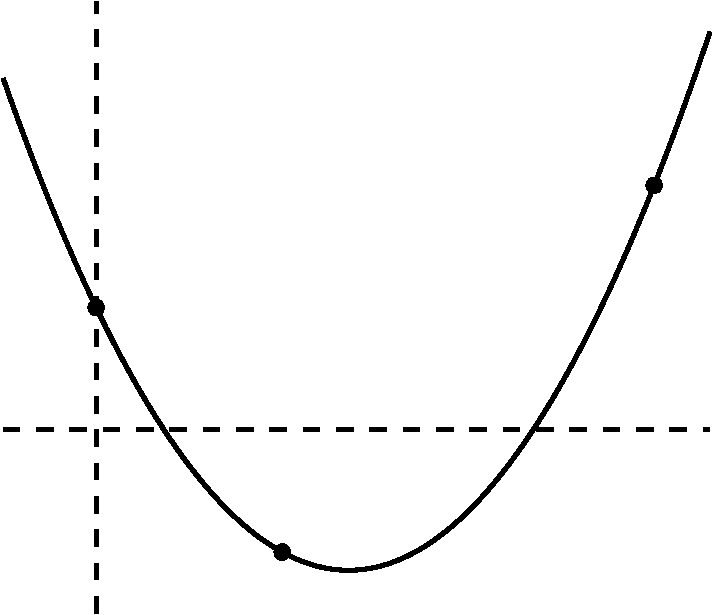
\includegraphics[width=0.4\textwidth]{figs/mar21fig1.pdf}

\bigskip\bigskip
\prob{2} \textbf{line least-squares fits 4 points}

\msni data $(x,y)$: $(0,1)$, $(1,-1)$, $(1.5,0.5)$, $(3,2)$

\msni curve: $p(x) = v_1 + v_2 x$

\msni solved: $A^\top A \bv = A^\top \bb$

\msni $\ds A = \begin{bmatrix} 1 & 0 \\ 1 & 1 \\ 1 & 1.5 \\ 1 & 3 \end{bmatrix}$, \quad $\ds \bb = \begin{bmatrix} 1 \\ -1 \\ 0.5 \\ 2 \end{bmatrix}$

\msni $\implies$ \quad $\ds \bv = \begin{bmatrix} -4/75 \\ 37/75 \end{bmatrix}$

\vspace{-60mm}
\hfill 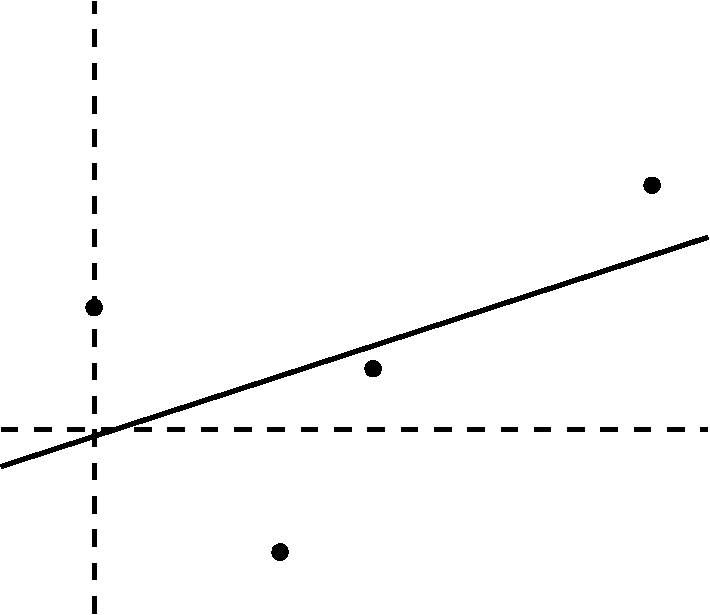
\includegraphics[width=0.4\textwidth]{figs/mar21fig2.pdf}
\vfill

\clearpage \newpage
\prob{3} \textbf{quadratic least-squares fits 6 points}

\msni data $(x,y)$: $(0,-1)$, $(0.5,0)$, $(1,2)$, $(1.5,2.5)$,

\qquad \qquad $(2.5,3)$, $(3,1)$

\msni curve: $p(x) = v_1 + v_2 x + v_2 x^2$

\msni solved: $A^\top A \bv = A^\top \bb$

\msni $\ds A = \begin{bmatrix} 1 & 0 & 0 \\ 1 & 0.5 & 0.25 \\ 1 & 1 & 1 \\ 1 & 1.5 & 2.25 \\ 1 & 2.5 & 6.25 \\ 1 & 3 & 9 \end{bmatrix}$, \quad $\ds \bb = \begin{bmatrix} -1 \\ 0 \\ 2 \\ 2.5 \\ 3 \\ 1 \end{bmatrix}$

\msni $\implies$ \quad $\ds \bv = \begin{bmatrix} -1.35238 \\ 4.40000 \\ -1.16190 \end{bmatrix}$

\vspace{-80mm}
\hfill 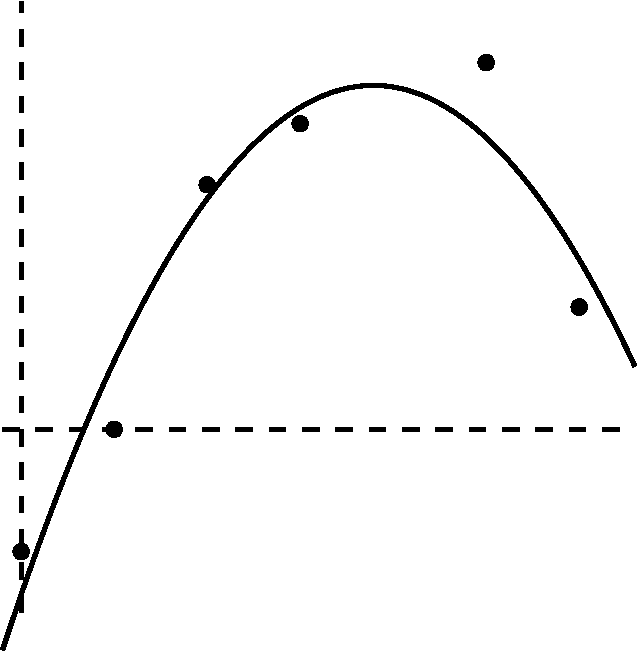
\includegraphics[width=0.4\textwidth]{figs/mar21fig3.pdf}

\vspace{20mm}

\prob{4} \textbf{trigonometric least-squares fits 6 points}

\msni data $(x,y)$: $(0,-1)$, $(0.5,0)$, $(1,2)$, $(1.5,2.5)$,

\qquad \qquad $(2.5,3)$, $(3,1)$

\msni curve: $p(x) = v_1 + v_2 \sin x + v_2 \cos x$

\msni solved: $A^\top A \bv = A^\top \bb$

\msni $\ds A = \begin{bmatrix} 1 & \sin(0) & \cos(0) \\ 1 & \sin(0.5) & \cos(0.5) \\ 1 & \sin(1) & \cos(1) \\ 1 & \sin(1.5) & \cos(1.5) \\ 1 & \sin(2.5) & \cos(2.5) \\ 1 & \sin(3) & \cos(3) \end{bmatrix}$, \quad $\ds \bb = \begin{bmatrix} -1 \\ 0 \\ 2 \\ 2.5 \\ 3 \\ 1 \end{bmatrix}$

\msni $\implies$ \quad $\ds \bv = \begin{bmatrix} -0.15410 \\ 3.00287 \\ -1.08695 \end{bmatrix}$

\vspace{-60mm}
\hfill 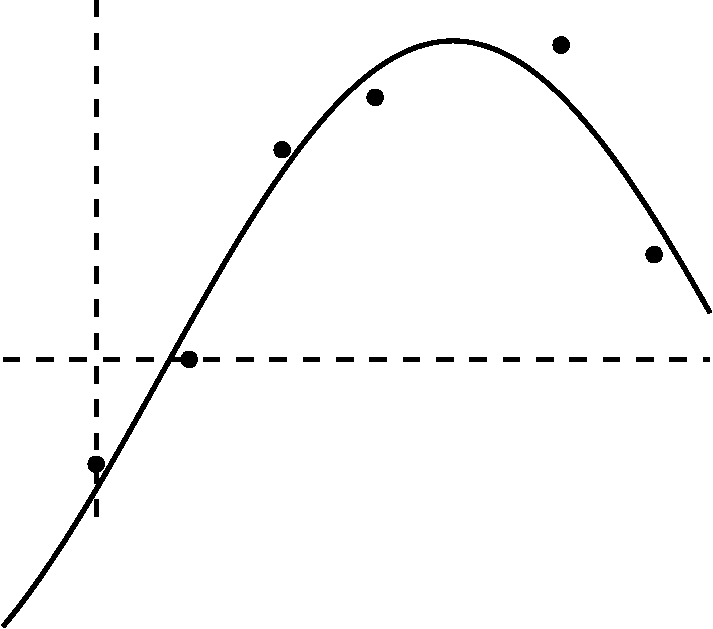
\includegraphics[width=0.4\textwidth]{figs/mar21fig4.pdf}
\vfill
\end{document}
